% Preamble
% ---
\documentclass{article}

% Packages
% ---
\usepackage{amsmath} % Advanced math typesetting
\usepackage[utf8]{inputenc} % Unicode support (Umlauts etc.)
\usepackage[ngerman]{babel} % Change hyphenation rules
\usepackage{hyperref} % Add a link to your document
\usepackage{graphicx} % Add pictures to your document
\usepackage{listings} % Source code formatting and highlighting
\usepackage{booktabs}

\renewcommand{\figurename}{Figure}
%\usepackage[labelsep=endash]{caption}

\usepackage{xcolor}
\lstset { %
    language=C++,
    backgroundcolor=\color{black!5}, % set backgroundcolor
    basicstyle=\footnotesize,% basic font setting
}



\title{%
	MA226 : Monte-Carlo Simulation\\
	 Geometric Brownian Motion\\
	 \large Assignment 11}

\date{13-04-2017}

\author{%
	Turkhade Hrushikesh Pramod\\
	150123044	}	

\begin{document}

	\maketitle
	\pagenumbering{gobble}
	
	\newpage
	\pagenumbering{arabic}
	
	\section{Problem 1}
	\paragraph{}
		We have to generate 10 sample paths from geometric brownian motion and plot them for various values of $\mu$ and $\sigma$.
		
	\paragraph{}
	\[S(t_{i+1}) = S(t_i)e^{((t_{i+1}-t_{i})[\mu- \frac{{\sigma^{2}}}{2}] + \sigma \sqrt{t_{i+1}-t_i}.Z_{i+1})}\]
	
	\paragraph{}
	Values of $\mu$ used are $0.06$ and $-0.06$.
	Values of $\sigma$ used are $0.3$ and $0.4$.
		
	\subsection{Source code of the solution}
		\lstinputlisting[language=R,firstline=1]{code/que1.R}

	\clearpage

		\subsection{Plots}
	
		\paragraph{}
		In the following plots, each color represents unique brownian path.
		
			\begin{figure}[!ht]
  			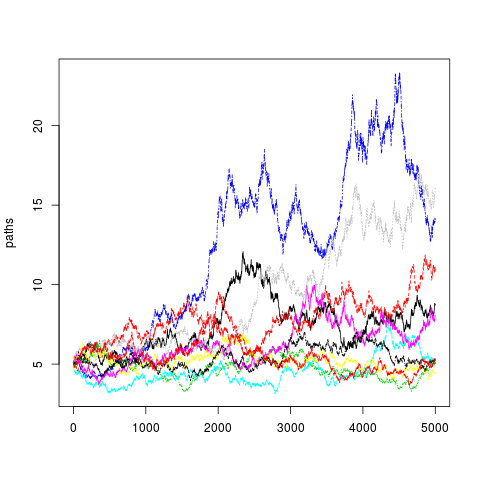
\includegraphics[width=\linewidth]{pic/que1_1.png}
 			 \caption{Paths for Geometric Brownian Motion for $\mu=0.06$ and $\sigma=0.3$.}
  			\label{fig:hist1_1}
		\end{figure}
		
		\begin{figure}[!ht]
  			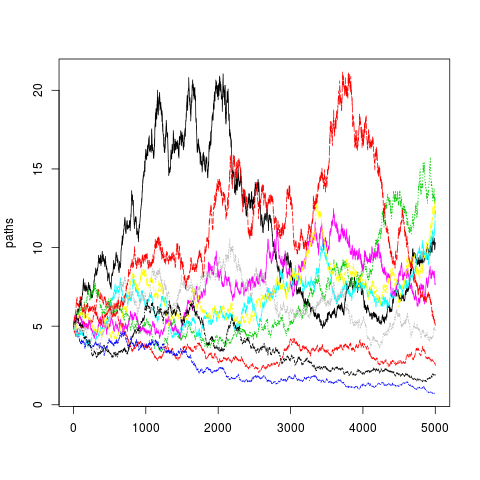
\includegraphics[width=\linewidth]{pic/que1_2.png}
 			 \caption{Paths for Geometric Brownian Motion for $\mu=0.06$ and $\sigma=0.3$.}
  			\label{fig:hist1_1}
		\end{figure}
		
		\begin{figure}[!ht]
  			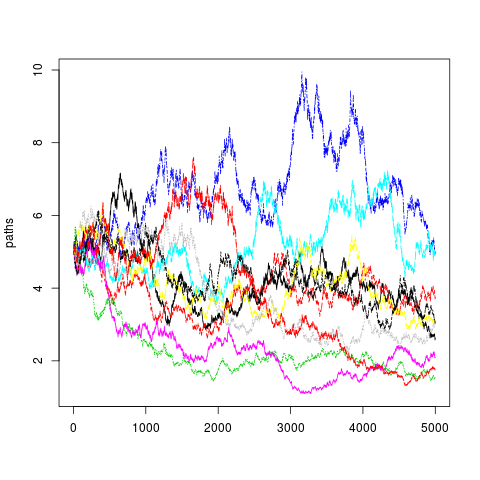
\includegraphics[width=\linewidth]{pic/que2_1.png}
 			 \caption{Paths for Geometric Brownian Motion for $\mu=-0.06$ and $\sigma=0.4$.}
  			\label{fig:hist1_1}
		\end{figure}
		
		\begin{figure}[!ht]
  			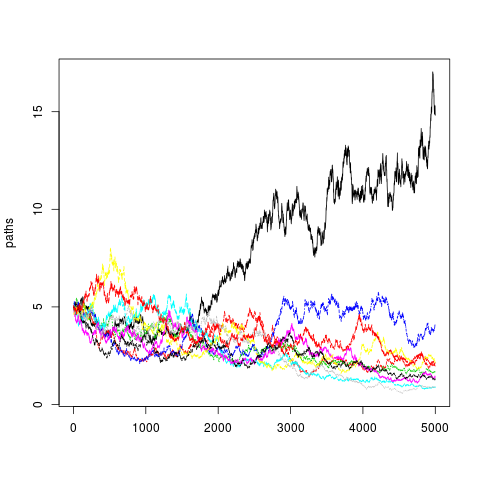
\includegraphics[width=\linewidth]{pic/que2_2.png}
 			 \caption{Paths for Geometric Brownian Motion for $\mu=-0.06$ and $\sigma=0.4$.}
  			\label{fig:hist1_1}
		\end{figure}
		
		\clearpage
	
		
	
	\section{Problem 2}
	\paragraph{}
		We have to generate 1000 sample paths from geometric brownian motion and verify observed expectation and vaiance and theoritical expection and variance.
		
	
	\subsection{Source code of the solution}
		\lstinputlisting[language=R,firstline=1]{code/que2.R}
		
	
		\subsection{Observation}

For mu= 0.06 and sigma= 0.3 \\
Observed Expectation =  6.800481 \\
Observed Variance =  29.58148 \\
Theoritical Expection =  6.749294 \\
Theoritical Variance =  25.88831 \\
\\
For mu= 0.06 and sigma= 0.4 \\
Observed Expectation =  6.822147 \\
Observed Variance =  47.73617 \\
Theoritical Expection =  6.749294 \\
Theoritical Variance =  55.82703 \\
\\
For mu= -0.06 and sigma= 0.3 \\
Observed Expectation =  3.678885 \\
Observed Variance =  7.376168 \\
Theoritical Expection =  3.704091 \\
Theoritical Variance =  7.797409 \\
\\
For mu= -0.06 and sigma= 0.4 \\
Observed Expectation =  3.665376 \\
Observed Variance =  14.21604 \\
Theoritical Expection =  3.704091 \\
Theoritical Variance =  16.81478\\
	
		

\end{document}